\subsection{Come un'azienda genera reddito}
Il reddito di impresa è il profitto economico realizzato dall’esercizio di un’attività economica e richiede l’impiego di risorse umane, di mezzi, di attrezzature e di tutto ciò che occorre per produrre beni o servizi.

Il reddito d’impresa è la differenza tra le componenti positive e le componenti negative del reddito stesso.

Le componenti positive di reddito sono:
\begin{itemize}
	\item ricavi: realizzati dalle vendite di beni o servizi durante l’esercizio
	\item plusvalenze patrimoniali: vendita di un macchinario usato ad un valore superiore al suo valore contabile
	\item sopravvenienze attive: rinuncia ad incassare un credito da parte di un fornitore
	\item proventi finanziari: interessi attivi maturati sui conti correnti bancari o postali, o sui crediti verso clienti o soggetti diversi
	\item rivalutazioni: di immobili, di quote azionarie, ecc...
	\item variazione positiva delle rimanenze finali di merci, prodotti finiti, semilavorati, materie prime, rispetto alle loro esistenze iniziali
\end{itemize}

Mentre le componenti negative di reddito sono:
\begin{itemize}
	\item costi: costi di acquisto delle merci, costi del personale ecc...
	\item minusvalenze patrimoniali: vendita di un impianto usato ad un valore inferiore al suo valore contabile
	\item sopravvenienze passive: una multa, un risarcimento a terzi
	\item oneri finanziari: interessi passivi che maturano su debiti verso le banche, i fornitori, ecc...
	\item ammortamenti: quota del costo d’acquisto di alcuni beni aziendali ad utilità pluriennale che si fa incidere sul reddito dell’esercizio
	\item accantonamenti: quote di costi che si fanno pesare sul reddito d’esercizio in previsione di eventi futuri (es. quota fondo \textit{TFR})
	\item svalutazioni: di immobili, di quote azionarie, ecc...
	\item imposte: alcuni tipi di imposte correnti e differite, in misura totale o parziale
\end{itemize}

\begin{center}

\begin{figure}[H]
	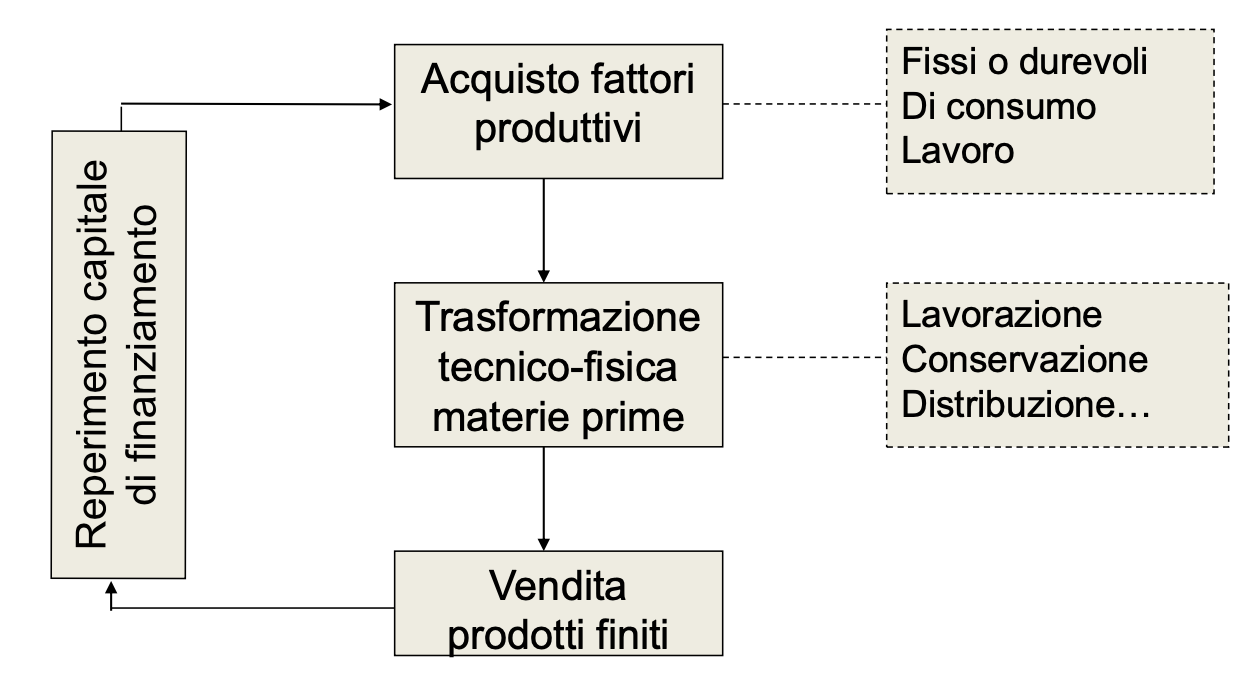
\includegraphics[width=0.8\linewidth]{resources/chapters/Bilancio/images/vita-impresa.png}
	\centering
	\caption{Modello rappresentate la vita di un'impresa}
\end{figure}

\begin{figure}[H]
	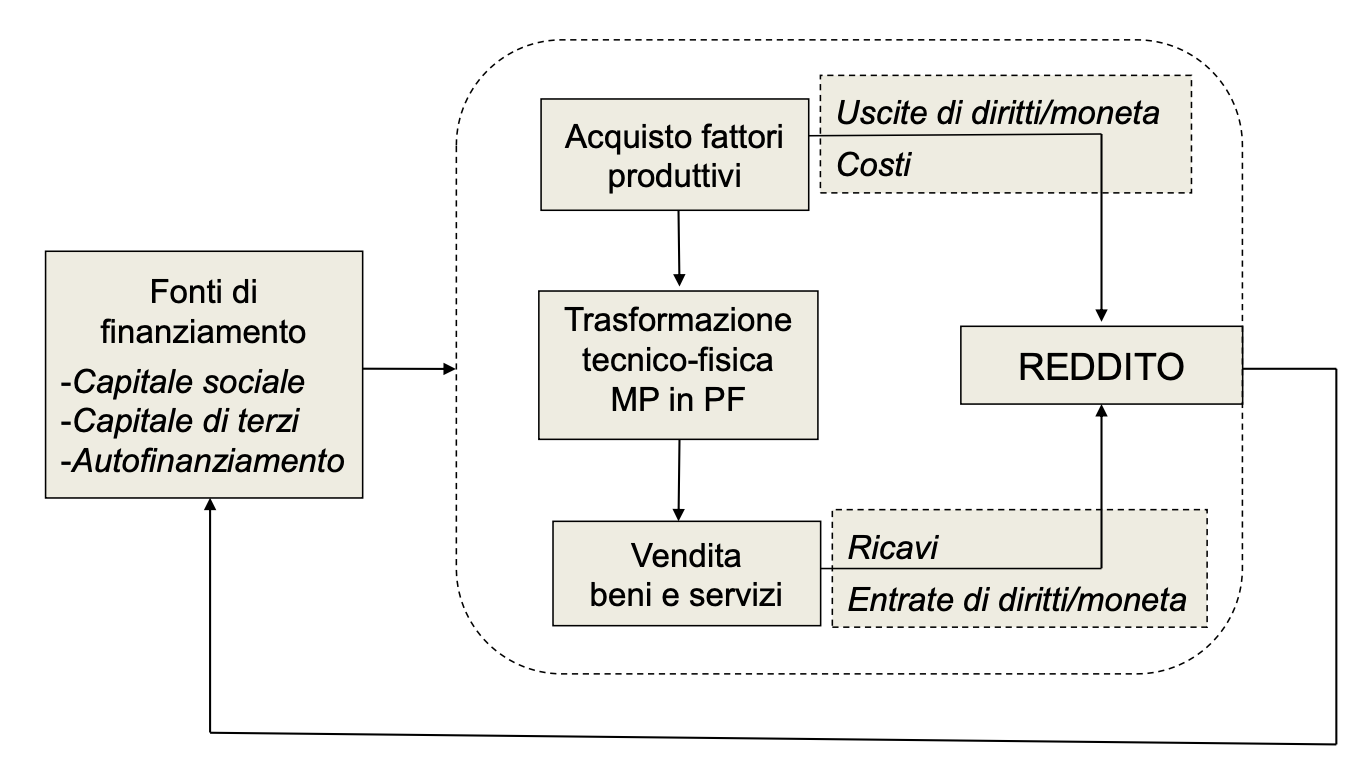
\includegraphics[width=0.8\linewidth]{resources/chapters/Bilancio/images/modello-economico-finanziario.png}
	\centering
	\caption{Modello rappresentate il modello Economico-Finanziario di un'impresa}
\end{figure}
\end{center}


\subsection{Aspetti economici e patrimoniali dello scambio}
\begin{table}[h!]
	\begin{tabular}{|c | c | c|}
		\hline
		& Cessione di beni/servizi & Acquisizione di beni/servizi \\
		\hline
		Aspetto economico & Ricavo & Costo \\
		\hline
		Aspetto patrimoniale & & \\
		- finanziario & Credito & Debito \\
		- economico & Entrata di moneta & Uscita di moneta \\
		\hline
	\end{tabular}
	\centering
	\caption{Schematizzazione modello economico-finanziario}
\end{table}

\subsection{Capitale di Rischio e di Prestito}
Il capitale di rischio, detto anche capitale proprio, rappresenta:
\begin{itemize}
	\item conferimento dei soci/imprenditore
	\item senza obbligo di restituzione
	\item momenti differenti
	\item remunerazione (dipendente dai risultati oggettivi, autofinanziamento)
\end{itemize}
Il capitale di prestito, detto anche capitale di terzi, rappresenta:
\begin{itemize}
	\item oneri (interessi) per la disponibilità temporanea
	\item rimborso a scadenze prefissate
	\item nel caso di mancata restituzione, i finanziatori possono anche richiedere il fallimento
\end{itemize}

\subsection{Acquisti di fattori produttivi}

L’acquisto dei fattori produttivi rappresenta la fase della gestione aziendale in cui l’impresa compie gli investimenti necessari alla realizzazione del processo produttivo.

L’acquisto dei fattori produttivi viene effettuato sui mercati di approvvigionamento e rappresenta un’operazione di investimento che genera costi. I fattori produttivi vengono classificati in: \textit{beni strumentali, merci e materie di consumo, servizi}. 
\subsubsection{Elementi che caratterizzano lo scambio}
Gli elementi che caratterizzano lo scambio sono:
\begin{itemize}
	\item L’oggetto (che cosa?)
		\begin{itemize}
			\item Risorse ricevute (= fattori produttivi):
				\begin{itemize}
					\item Materiali e prodotti
					\item Macchinari e impianti
					\item Lavoro
					\item Servizi
					\item Conoscenze (brevetti, licenze, know-how)
					\item Mezzi monetari (moneta e assimilabili)
				\end{itemize}
			\item risorse cedute: beni o servizi
		\end{itemize}
	\item Soggetti terzi (con chi?)
		\begin{itemize}
			\item Clienti
			\item Fornitori
			\item Finanziatori
			\item Azionisti o proprietari
			\item Pubbliche istituzioni
		\end{itemize}
	\item Ccontropartita (in cambio di che cosa?): a fronte del passaggio di proprietà della risorsa oggetto di scambio si ha la
   una remunerazione della risorsa stessa in denaro o diritti
\end{itemize}
